% A simple template for LaTeX documents
% 
% To produce pdf run:
%   $ pdflatex paper.tex 
%

\documentclass[12pt]{article}

% Begin paragraphs with new line
\usepackage{parskip}  

% Change margin size
\usepackage[margin=1in]{geometry}   

% Graphics Example:  (PDF's make for good plots)
\usepackage{graphicx}               
% \centerline{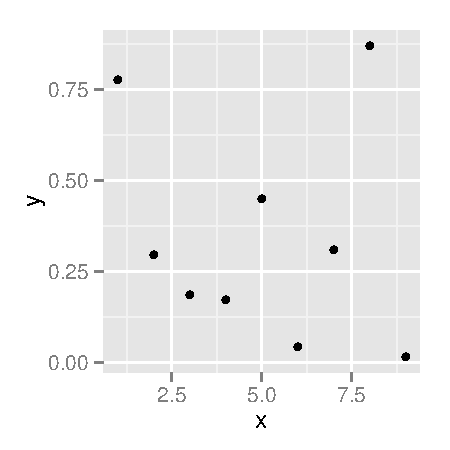
\includegraphics{figure.pdf}}

% Allows hyperlinks
\usepackage{hyperref}

% Blocks of code
\usepackage{listings}
\lstset{basicstyle=\ttfamily, title=\lstname}
% Insert code like this. replace `plot.R` with file name.
% \lstinputlisting{plot.R}

% Supports proof environment
\usepackage{amsthm}

% Allows writing \implies and align*
\usepackage{amsmath}

% Allows mathbb{R}
\usepackage{amsfonts}

% Allows alpha labels rather than numeric
\usepackage{enumitem}


%%%%%%%%%%%%%%%%%%%%%%%%%%%%%%%%%%%%%%%%%%%%%%%%%%%%%%%%%%%%

\begin{document}

\begin{center}
    {\Large Homework 1}\\
    \bigskip
    \bigskip
    \hrule
    \medskip
    Clark Fitzgerald\\
    Stats 206
\end{center}

\subsubsection*{2. True / False}
\begin{enumerate}[label=\alph*]
\item  \textbf{True} The least squares line always passes the center of the data.
This is implied by the formula
\[
    \hat{\beta_0} = \bar{Y} - \hat{\beta_1} \bar{X}.
\]
The large point in the below plot is the center of the data.

\centerline{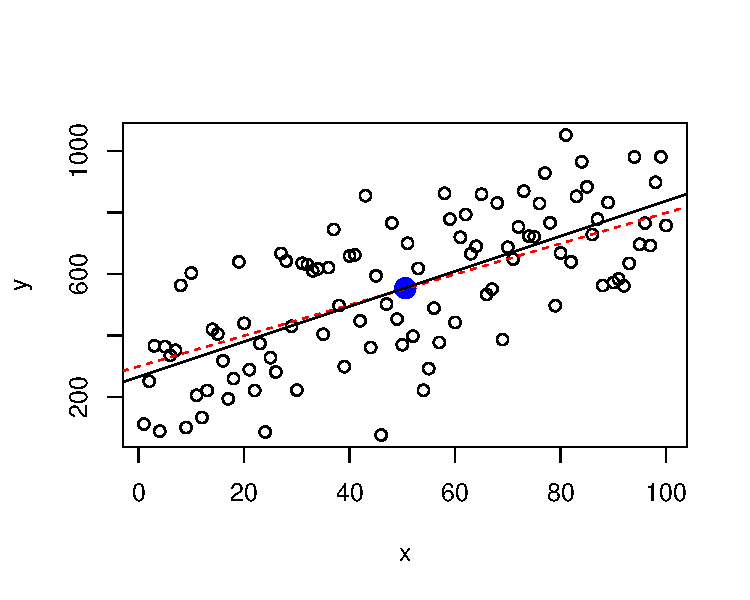
\includegraphics{regress.pdf}}

\item \textbf{False} The least squares line fits the data
best by definition. All other lines, including the true line, are worse
than the least square lines in this respect. 
In the figure above the fitted regression line is the solid line,
while the true regression line is the dashed line. They are not the same.

\item \textbf{True} $\bar{X} = 0$ and $\bar{Y} = 0 \implies \hat{\beta_0} =
0$. This is implied by the equation in part a).

\item \textbf{True} Standard errors of $\beta_i$. 

\item \textbf{True} It's harder to predict than to infer the mean.

\item \textbf{True} A 95\% confidence interval represents our confidence that
the true value lies in that interval.

\item \textbf{True} One sided and two sided t tests are different, for
example.

\item \textbf{True} For most data sets there are generally fewer data points far from the mean,
which makes estimation more difficult. 

\item \textbf{True} Assuming that the regression coefficients are well 
defined, the least squares line will interpolate collinear points. This
implies that $y_i = \hat{y_i}$ for all $y_i \implies SSR = SSTO \implies R^2 = 1$.

\item \textbf{False} A small $R^2$ does not mean that the predictor and
response are not related; the relationship may be nonlinear. In the graph
below the points were generated from a sine function plus random normal
noise. The $R^2$ for the fitted line is nearly 0.

\centerline{\includegraphics{nonlinear.pdf}}

\item \textbf{True} Scatter plots show nonlinear relationships between two
variables. The sine function is easily recognized above. However, if they are done incorrectly they won't show the
relationship, for example plotting tens of thousands of filled points without adjusting the
alpha value. Then the graph becomes a big uninformative blob.

\end{enumerate}

\end{document}
